\documentclass[a4paper, 12pt]{article}        % General format
%\documentclass[a4paper, 14pt]{extarticle}    % Advanced format

%%%% Charset
\usepackage{cmap}                             % Make PDF files searchable and copyable
\usepackage[utf8x]{inputenc}                  % Accept different input encodings
\usepackage[T2A]{fontenc}                     % Russian font
\usepackage[russian]{babel}                   % Multilingual support (T2A)

%%%% Graphics
\usepackage[dvipsnames]{xcolor}               % Driver-independent color extensions
\usepackage{graphicx}                         % Enhanced support for graphics
\usepackage{wrapfig}                          % Produces figures which text can flow around

%%%% Graphs
\usepackage{tikz}                             % Creating graphics programmatically
\usetikzlibrary{arrows}                       % Arrows for tikz

%%%% Math
\usepackage{amsmath}                          % American Mathematical Society (AMS) math facilities
\usepackage{amsfonts}                         % fonts from the AMS
\usepackage{amssymb}                          % additional math symbols

%%%% Typography (don't forget about cm-super)
\usepackage{microtype}                        % subliminal refinements towards typographical perfection
\linespread{1.3}                              % line spacing
\usepackage[left=2.5cm, right=1.5cm, top=2.5cm, bottom=2.5cm]{geometry}
\setlength{\parindent}{0pt}                   % we don't want any paragraph indentation
\usepackage{parskip}                          % add distance between paragraphs

%%%% Tables
\usepackage{tabularx}                         % Enhanced tables
\usepackage{multirow}                         % For tabular
\usepackage{hhline}                           % For tabular

%%%% Other
\usepackage{url}                              % Verbatim with URL-sensitive line breaks
\usepackage{fancyvrb}                         % Sophisticated verbatim text
\setcounter{secnumdepth}{5}                   % Turn on subsection numbering

%------------------------------------------------------------------------------
\usepackage{listings}                         % typeset source code listings

% Цвета для кода
\definecolor{mygreen}{HTML}{3F7F5F}           % color values Red, Green, Blue
\definecolor{mylilas}{RGB}{170,55,241}

% Настройки отображения кода
\lstset{language=Matlab,%
    %basicstyle=\color{red},
    breaklines    =  true,                    % Перенос длинных строк
    morekeywords  =  {matlab2tikz},           %
    keywordstyle  =  \color{blue},            %
    morekeywords  =  [2]{1},                  %
    keywordstyle  =  [2]{\color{black}},      %
    identifierstyle= \color{black},           %
    stringstyle   =  \color{mylilas},         %
    commentstyle  =  \color{mygreen},         %
    showstringspaces=false,                   % don't mark spaces in strings
    frame         =  tblr                     % draw a frame at all sides of the code block
    rulecolor     =  \color{frame},           % Цвет рамки
    tabsize       =  2,                       % tab space width
    showstringspaces=false,                   % don't mark spaces in strings
    numbers       =  left,                    %
    numberstyle   =  {\tiny \color{black}},   % size of the numbers
    numbersep     =  9pt,                     % this defines how far the numbers are from the text
    emph          =  [1]{for,end,break},      %
    emphstyle     =  [1]\color{red},          %some words to emphasise
    %emph         =  [2]{word1,word2},        %
    %emphstyle    =  [2]{style},              %
    extendedchars =  true,                    % Для отображения русского языка
    literate=
        {Ö}{{\"O}}1                    {Ä}{{\"A}}1                    {Ü}{{\"U}}1
        {ß}{{\ss}}1                    {ü}{{\"u}}1                    {ä}{{\"a}}1
        {ö}{{\"o}}1                    {~}{{\textasciitilde}}1        {а}{{\selectfont\char224}}1
        {б}{{\selectfont\char225}}1    {в}{{\selectfont\char226}}1    {г}{{\selectfont\char227}}1
        {д}{{\selectfont\char228}}1    {е}{{\selectfont\char229}}1    {ё}{{\"e}}1
        {ж}{{\selectfont\char230}}1    {з}{{\selectfont\char231}}1    {и}{{\selectfont\char232}}1
        {й}{{\selectfont\char233}}1    {к}{{\selectfont\char234}}1    {л}{{\selectfont\char235}}1
        {м}{{\selectfont\char236}}1    {н}{{\selectfont\char237}}1    {о}{{\selectfont\char238}}1
        {п}{{\selectfont\char239}}1    {р}{{\selectfont\char240}}1    {с}{{\selectfont\char241}}1
        {т}{{\selectfont\char242}}1    {у}{{\selectfont\char243}}1    {ф}{{\selectfont\char244}}1
        {х}{{\selectfont\char245}}1    {ц}{{\selectfont\char246}}1    {ч}{{\selectfont\char247}}1
        {ш}{{\selectfont\char248}}1    {щ}{{\selectfont\char249}}1    {ъ}{{\selectfont\char250}}1
        {ы}{{\selectfont\char251}}1    {ь}{{\selectfont\char252}}1    {э}{{\selectfont\char253}}1
        {ю}{{\selectfont\char254}}1    {я}{{\selectfont\char255}}1    {А}{{\selectfont\char192}}1
        {Б}{{\selectfont\char193}}1    {В}{{\selectfont\char194}}1    {Г}{{\selectfont\char195}}1
        {Д}{{\selectfont\char196}}1    {Е}{{\selectfont\char197}}1    {Ё}{{\"E}}1
        {Ж}{{\selectfont\char198}}1    {З}{{\selectfont\char199}}1    {И}{{\selectfont\char200}}1
        {Й}{{\selectfont\char201}}1    {К}{{\selectfont\char202}}1    {Л}{{\selectfont\char203}}1
        {М}{{\selectfont\char204}}1    {Н}{{\selectfont\char205}}1    {О}{{\selectfont\char206}}1
        {П}{{\selectfont\char207}}1    {Р}{{\selectfont\char208}}1    {С}{{\selectfont\char209}}1
        {Т}{{\selectfont\char210}}1    {У}{{\selectfont\char211}}1    {Ф}{{\selectfont\char212}}1
        {Х}{{\selectfont\char213}}1    {Ц}{{\selectfont\char214}}1    {Ч}{{\selectfont\char215}}1
        {Ш}{{\selectfont\char216}}1    {Щ}{{\selectfont\char217}}1    {Ъ}{{\selectfont\char218}}1
        {Ы}{{\selectfont\char219}}1    {Ь}{{\selectfont\char220}}1    {Э}{{\selectfont\char221}}1
        {Ю}{{\selectfont\char222}}1    {Я}{{\selectfont\char223}}1    {і}{{\selectfont\char105}}1
        {ї}{{\selectfont\char168}}1    {є}{{\selectfont\char185}}1    {ґ}{{\selectfont\char160}}1
        {І}{{\selectfont\char73}}1     {Ї}{{\selectfont\char136}}1    {Є}{{\selectfont\char153}}1
        {Ґ}{{\selectfont\char128}}1
}

\usepackage{caption}                          % Для настройки заголовка кода
\DeclareCaptionFont{white}{\color{сaptiontext}}
\DeclareCaptionFormat{listing}{\parbox{\linewidth}{\colorbox{сaptionbk}{\parbox{\linewidth}{#1#2#3}}\vskip-4pt}}
%\captionsetup[lstlisting]{format=listing,labelfont=white,textfont=white}
\renewcommand{\lstlistingname}{Листинг}       % Переименование Listings в нужное именование структуры
%------------------------------------------------------------------------------

\begin{document}

%------------------------------------------------
\begin{titlepage}
\thispagestyle{empty}

\begin{center}
Санкт-Петербургский политехнический университет Петра Великого\\
Институт Информационных Технологий и Управления \\*
Кафедра компьютерных систем и программных технологий \\*
\hrulefill
\end{center}

\vspace{15em}

\begin{center}
\Large Отчёт по практической работе\\по предмету «Системное программное обеспечение» \\
\end{center}

\vspace{1em}

% \linebreak
\begin{center}
\textsc{\textbf{Процесс загрузки операционной системы Linux}}
\end{center}

\vspace{20em}

\begin{flushleft}
Работу выполнил студент гр. 53501/3 \hrulefill Мартынов С. А. \\
\vspace{1.5em}
Работу принял преподаватель \hrulefill Душутина Е. В. \\
\end{flushleft}

\vspace{\fill}

\begin{center}
Санкт-Петербург \\
2015
\end{center}

\end{titlepage}
%------------------------------------------------
\setcounter{page}{2} % Титульная страница
\tableofcontents

%------------------------------------------------------------------------------

\newpage
\section*{Введение}
\addcontentsline{toc}{section}{Введение}

Драйвер устройства -- это низкоуровневая программа, содержащая специфический код для работы с устройством, которая позволяет пользовательским программам (и самой ОС) управлять им стандартным образом.

В современных версиях ядра Linux по умолчанию присутствуют все необходимые драйверы для всех поддерживаемых устройств\cite{Love}. Но для старых версий ядра иногда приходится заниматься бэк-портированием драйверов или даже написанием из с нуля, чтобы обеспечить корректную работу железа.

Все устройства можно разделить на:
\begin{itemize}
\item \textbf{Символьные}. Чтение и запись устройства идет посимвольно. Примеры таких устройств: клавиатура, последовательные порты.
\item \textbf{Блочные}. Чтение и запись устройства возможны только блоками, обычно по 512 или 1024 байта. Пример - жесткий диск.
\item \textbf{Сетевые интерфейсы}. Отличаются тем, что не отображаются на файловую систему, т.е. не имеют соответствующих файлов в директории /dev, поскольку из-за специфики этих устройств работа с сетевыми устройствами как с файлами неэффективна. Пример - сетевая карта (eth0).
\end{itemize}

В распоряжении имеется относительно старая материнская плата ASUS P5B на чипсете Intel P965, со встроенной сетевой картой на основе Realtek RTL8111B, для которой будет разработан драйвер, работающий в старой версии ядра Linux.

Это довольно популярная платформа r8169, для которой открыта спецификация. Ссылка на неё приводится в списке использованных материалов. % Введение

\newpage
\section{BIOS}

При включении питания компьютера, в его оперативной памяти отсутствуют какие-либо данные, поэтому управление компьютером может осуществляться только аппаратным обеспечением. На Intel-овских платформах начальная загрузка операционной системы осуществляется посредством так называемой "базовой системы ввода/вывода" или BIOS.

После включения компьютера блок питания проверяет все необходимые уровни напряжений. Если все уровни напряжений соответствуют номинальным, то на материнскую плату поступит сигнал PowerGood. До появления этого сигнала на вход процессора подается сигнал RESET, который удерживает процессор в сброшенном состоянии. Но после получения сигнала PowerGood от блока питания сигнал RESET будет снят и процессор начнет выполнять свои первые инструкции. При этом процессор стартует от вполне известного состояния: командный регистр CS содержит 0xFFFF, указатель команд (регистр IP) содержит 0, сегментные регистры данных и стека содержат 0. Таким образом, после снятия RESET процессор в реальном режиме выполняет инструкции, размещающиеся в области ROM BIOS, начинающейся с адреса FFFF:0000 (физический адрес, соответственно, - 0xFFFF0). Размер этой области, очевидно, составляет 16 байт, вплоть до конца максимально адресуемого адресного пространства в реальном режиме - 0xFFFFF. По этому адресу располагается инструкция перехода на реально исполняемый код BIOS.

По соображениям снижения стоимости код BIOS в относительно современных материнских платах хранится в постоянной памяти (ПЗУ) в сжатом виде. Только небольшая его часть, используемая на самых первых этапах загрузки, является непосредственно исполняемой. Поэтому первая задача, которая решается сразу после включения питания, заключается в том, чтобы инициализировать контроллер DRAM, декомпрессировать основной код BIOS и загрузить его в ту область оперативной памяти (RAM), которую именуют "теневой" (shadow RAM).

Эта область затем защищается от записи и управление передается на записанный в нее исполняемый код BIOS. Теневая память в ходе дальнейшей работы отдана в полное владение чипсета материнской платы; операционная система к ней доступа не имеет. Но аппаратными средствами обеспечивается отображение теневой памяти на те области, которые в реальном режиме работы доступны для старых операционных систем типа MS-DOS, так что последние обнаруживают код BIOS именно там, где ожидают его найти.

Исполняемый код BIOS вначале реализует функцию начального самотестирования (POST - Power-On Self Test). При этом тестируются процессор, память и системные средства ввода/вывода, а также производится конфигурирование программно-управляемых аппаратных средств компьютера. Кроме того производится поиск и обнаружение периферийных устройств. При этом производится сравнение установок, записанных в CMOS (Complementary Metal Oxide Semiconductor) с тем, что реально обнаружено в системе. Некоторые несовпадения, например, различие типов флоппи-дисковода, могут быть допустимы и процесс загрузки продолжится. Другие ошибки, например, отсутствие видеокарты, приводят к невозможности дальнейшей загрузки. Но все сообщения о выявленных на этом этапе ошибках сводятся только к тому, что раздастся несколько коротких звуковых сигналов (каждый вендор имеет свой код звуковых ошибок, который нужно смотреть по документации на материнскую плату).

Некоторые типы периферийных устройств могут содержать расширения BIOS в собственных ПЗУ. В таком случае устанавливаются соответствующие ссылки на эти расширения. Основная причина, по которой это необходимо, заключается в том, что по историческим причинам размер первичного загрузчика (загрузчика первого этапа) на персональных компьютерах ограничен величиной 446 байт. Этого явно недостаточно для того, чтобы включить в этот загрузчик драйверы всех периферийных устройств (например, дисплея и устройств хранения данных), которые могут понадобиться на этапе начальной загрузки системы. Тем более, что драйверы могут различаться для однотипных устройств от разных производителей. Поэтому функция загрузки некоторых драйверов возлагается на BIOS.

После завершения процедуры самотестирования та часть кода BIOS, которая реализует процедуры самотестирования (POST), удаляется из оперативной памяти. Оставшаяся часть BIOS, реализующая функции BIOS (runtime services), остается в ОП. Она будет доступна в последующем для загруженной операционной системы.

Первой задачей той части BIOS, которая осталась в ОП, является поиск активного загрузочного устройства. Список устройств, которые могут являться загрузочными, хранится в энергонезависимой памяти компьютера (CMOS), а порядок просмотра этого списка является одним из настраиваемых параметров BIOS. Загрузочным устройством может быть дискета, CD-ROM, раздел жесткого диска, сетевое устройство или даже USB-устройство (флеш-диск). Поиск загрузочного устройства осуществляется путем вызова прерывания INT19h BIOS.

Процедура обработки прерывания INT19h состоит в том, что считывается сектор с координатами Cylinder:0 Head:0 Sector:1 на очередном устройстве, его содержимое помещается в ОП по адресу 0000:7С00h, после чего осуществляется проверка, является ли этот сектор загрузочным, то есть содержит ли он код первичного загрузчика. Загрузочные сектора помечаются "волшебным" числом 0x55AA в позиции 0x1FE = 510. Это последние два байта сектора. Наличие (или отсутствие) такого кода в последних байтах сектора позволяет программе BIOS решить, является ли данное устройство загрузочным.

Как только программа обработки прерывания обнаружит, что загруженный в память сектор содержит это самое "магическое число" 0x55AA, управление передается на начало этого сектора (по абсолютному адресу 0000:7С00h). Дальнейшие события зависят от того, где обнаружен загрузочный сектор - на жестком диске или на одном из других устройств: дискете, CD или flash-диске (на всех этих устройствах обычно создается образ загрузочной дискеты).

Если при проверке загрузочный сектор не обнаружен ни на одном устройстве, вызывается прерывание INT18h. Когда-то (в первых персональных компьютерах, производимых компанией IBM) это прерывание служило для вызова интерпретатора ROM-BASIC, который дальше управлял работой компьютера. Клоны IBM-PC не имеют BASIC в ROM-памяти и теперь это прерывание используют для организации загрузки по сети. Но мы не будем рассматривать эту ветку развития событий и вернемся к тому случаю, когда прерывание INT19h обнаружило загрузочный диск и передало управление находящейся в нем программе.

Примечание: Как следует из приведенного выше описания, BIOS выполняет массу работы по тестированию системы. Ядро Linux потом повторно проделывает всю эту работу. Как правило, после загрузки ядра большинство функций BIOS не используется (хотя есть некоторые исключения) и, тем не менее, этот уже бесполезный код BIOS сохраняется в "теневой" памяти компьютера.

\newpage
\section{Master Boot Record и Boot Record}

После того, как BIOS нашел загрузочное устройство, он передаёт управление программе, которая находилась в самом первом секторе этого диска или дискеты (физический адрес: цилиндр 0, головка 0, сектор 1). Теперь эта программа загружена в память и именно она управляет ходом дальнейшей загрузки. Со времен MS-DOS эту программу принято называть загрузочной записью (Boot Record), а первый сектор любого диска или дискеты - загрузочным сектором (Boot Sector).

Размер сектора на устройствах хранения данных равен 512 байтам. Существует три варианта загрузки ядра Linux[Т.Айвазяна]:
\begin{itemize}
\item с помощью загрузочного сектора Linux, загружающего непосредственно ядро (этот загрузочный сектор);
\item с помощью специального загрузчика типа LILO или GRUB;
\item с помощью программ, загружающих Linux из другой ОС.
\end{itemize}
Рассматривать только второй вариант, как наиболее распространенный.

С появлением жестких дисков большого объема, которые стали разбивать на разделы, небольшой загрузчик, размещаемый в загрузочном секторе и загружающий непосредственно ядро, перестал справляться с возросшим объемом задач. Надо было не просто загрузить файл с определенного физического адреса, но и найти загрузочный раздел перед этим. К тому же часть места, отведенного для загрузочной записи, отняла таблица разделов жесткого диска. Поэтому старая загрузочная запись была перенесена в первый сектор так называемого "активного" раздела, а в самый первый сектор на жестком диске стали записывать другую программу, задачей которой было найти "активный" раздел и загрузить программу из этого раздела. Первый сектор жесткого диска стали называть главным загрузочным сектором (а соответствующую программу - главной загрузочной записью или Master Boot Record, MBR). На жёстком диске MBR находится по тому же физическому адресу, что и BOOT-сектор на дискете (цилиндр 0, сторона 0, сектор 1). Его структура представлена в табл. 1

\begin{table}
\centering
\begin{tabular}{|c|c|c|}
\hline 
Смещение & Размер & Содержание \\ 
\hline 
0x000 & 446 байт & {Главная загрузочная запись (Master Boot Record)} \\ 
\hline 
0x1BE & 64 байта & Таблица разбиения диска \\ 
\hline 
0x1FE & 2 байта & "Магическое число" (0x55AA) \\ 
\hline 
\end{tabular}
\caption{Структура главного загрузочного сектора.}
\label{tab:xyz}
\end{table}

Это "Магическое число" 0x55AA, является признаком того, что диск является загрузочным. Содержащаяся в MBR такого диска таблица разбиения определяет 4 первичных раздела жесткого диска. Первые 446 байт MBR содержат небольшую программу, а также текст сообщений об ошибках, которые могут возникнуть в ходе ее выполнения.

Основная задача главной загрузочной записи состоит в том, чтобы найти и загрузить в оперативную память собственно загрузчик операционной системы. MBR сканирует таблицу разделов (partition table) в поисках первого (обычно он и единственный) активного раздела (раздела, помеченного как "загрузочный"). Если в таблице разделов активный раздел не обнаружен или хотя бы один раздел содержит неправильную метку, а также если несколько разделов помечены как активные, выдаётся соответствующее сообщение об ошибке. Когда активный раздел найден, программа считывает в оперативную память первый сектор активного раздела.

Практически все загрузчики современных операционных систем состоят из двух частей: загрузчика первого этапа (или первичного загрузчика), который имеет достаточно малый размер, чтобы разместиться в загрузочном секторе, и значительно большего по объему загрузчика 2-го этапа (или вторичного загрузчика), который может храниться уже где угодно на загрузочном носителе, обычно в разделе, содержащем корневую файловую систему. Загрузчик первого этапа может быть размещен как в главном загрузочном секторе диска, так и в загрузочном секторе активного раздела. Если вам приходилось устанавливать Linux, вы знаете, что программа инсталляции предоставляет пользователю такой выбор. Будем пока для определенности считать, что загрузчик 1-го этапа мы поместили в первый сектор активного раздела.

Итак, главная загрузочная запись отыскала активный раздел и загрузила из него в память загрузчик первого этапа, который теперь отвечает за продолжение процесса загрузки. Загрузчик первого этапа имеет такой же небольшой размер, как и код загрузочной записи диска, то есть не более 446 байт. Поэтому и сделать он может не больше, а именно - только загрузить основной загрузчик. Еще более затрудняет ситуацию то, код загрузчика первого этапа пока не имеет доступа к файловой системе и, следовательно, определяет расположение программ на диске, используя только информацию о физических секторах и низкоуровневые вызовы BIOS. Поэтому эта программа имеет единственной целью -- загрузку и запуск на выполнение загрузчика второго этапа.

\newpage
\section{Загрузчик 2 этапа операционной системы}

Итак, отработали маленькие программы, которые расположены в главной загрузочной записи диска (MBR) и в первом секторе активного раздела (Boot Record), то есть первичный загрузчик ОС. Код первичного загрузчика уже различен в разных операционных системах и является, частью загрузчика этой ОС (или какого-то универсального загрузчика, типа GRUB). Два основных загрузчика -- это LILO и GRUB. LILO (LInux LOader) -- это "родной" загрузчик операционной системы Linux, который, вытесняется универсальным загрузчиком GRUB (GRand Unified Bootloader).

Главная задача, которая стоит перед загрузчиком любой операционной системы, заключается в том, чтобы перенести в память ядро операционной системы и передать этому ядру управление дальнейшим функционированием компьютера. При этом современные загрузчики позволяют выбрать ядро из нескольких возможных вариантов как одной и той же операционной системы, так и загрузить ядра разных ОС. Некоторые загрузчики (в частности, GRUB) предоставляют пользователю возможность выполнения некоторых команд, то есть они представляют собой уже некоторое подобие командного процессора.

Одна из основных задач ядра -- управление железом, которое составляет аппаратную часть компьютера. Поэтому ядро после запуска производит опрос железа. Если драйвер найденного устройства вкомпилирован в ядро, устройство инициализируется. Однако стандартное ядро дистрибутива не может содержать драйверы для всех устройств, имеющихся в компьютере. Драйверы устройств, отсутствующие в ядре, надо загрузить из соответствующих файлов. После загрузки ядро должно запустить процесс init, который. Код программы init лежит где-то на носителе, доступ к которому тоже предоставляет файловая система.

Но файловая система не является частью ядра, драйвер файловой системы надо загрузить с того же диска. Корневая файловая система на загрузочном устройстве может быть самого разного типа (fat, ext2, reiserfs и так далее), может быть сжата, зашифрована. Получается замкнутый круг: чтобы подключить загрузочное устройство, надо получить доступ к файловой систем, а для этого надо подключить загрузочное устройство.

Решение этой проблемы было найдено за счет временного подключения виртуальной файловой системы, образ которой хранится в файле рядом с образом ядра. При этом минимальное число самых необходимых драйверов включается в само ядро, а все остальные размещаются на виртуальном диске, в виде подгружаемых модулей. Когда осуществляется загрузка (в частности, на неизвестном оборудовании) ядро опрашивает аппаратуру и загружает только те модули, которые соответствуют обнаруженной конфигурации. В частности, и LILO и GRUB создают в оперативной памяти виртуальный диск и разворачивают на нем временную корневую файловую систему, содержащую необходимые ядру драйверы устройств и служебные файлы. Сжатый образ этой файловой системы обычно располагается в одном каталоге с образом ядра в виде файла, содержащего дополнительные компоненты, например, драйверы некоторых устройств.

\newpage
\section{Загрузка и инициализация ядра}

Во время загрузки Linux на консоль выводится большое количество сообщений, в том числе и сообщений о действиях, выполняемых ядром при его инициализации. Эти сообщения обычно быстро проскакивают, и их невозможно прочитать. Ещё эти сообщения могут быть скрыты за заставкой. Но все эти сообщения сохраняются и их можно увидеть после завершения загрузки, воспользовавшись командой dmesg. Протоколирование этих сообщений осуществляется демоном протоколирования klogd (он запускается как один из потоков ядра). Klogd сохраняет эти сообщения в специальном буфере ядра, содержимое которого выдается по команде dmesg. Кроме того, klogd передает эти сообщения демону системного протоколирования syslogd, который записывает их в файл /var/log/messages. Благодаря этому они и доступны для просмотра и анализа после завершения запуска системы.

Ядро хранится на диске в сжатом виде. Только его первая часть не сжата. Когда загрузчик перенесет ядро в память, эта несжатая часть ядра выполняет декомпрессию оставшейся части. Несжатая часть кода, которая содержится в начале ядра, написана на ассемблере, ее можно найти в файлах arch/i386/boot/setup.S, arch/i386/boot/video.S и arch/i386/kernel/head.S.

Код, хранящийся в файлах arch/i386/boot/setup.S и arch/i386/boot/video.S, отвечает за получение системной информации от BIOS и размещение ее в подходящих местах системной памяти. Кратко перечислим основные действия, которые выполняет эта часть ядра:

\begin{itemize}
\item Проверка того, что ядро загружено правильно. Осуществляется проверкой сигнатуры в конце кода запуска. Если она не найдена, то копируются секторы с запускающим кодом и сигнатура ищется снова. Если опять безуспешно, то выдается сообщение "No setup signature found ...".
\item Проверка на возможность работы с верхней памятью. Если образ ядра слишком большой (и поэтому загружен в верхнюю память), а код несжатой части ядра не может работать с образами, расположенными в верхней памяти, то загрузка прекращается и выдачей сообщения "Wrong loader, giving up...".
\item Выяснение объема памяти системы. Для этого используется вызов трех различных функций BIOS: E820h, которая позволяет собрать карту памяти, затем E801h, которая вернет 32-битный размер памяти и последней вызывается 88h, которая вернет размер в диапазоне 0-64 МБ. Полученные значения сохраняются для дальнейшего использования.
\item Настройка режима видеоадаптера. Возможность выбора видеорежима зависит от конфигурации ядра. Можно указать специфичный (предопределенный) режим, который будет использован в процессе загрузки ядра, либо запросить меню со списком режимов, из которого пользователь выберет режим по своему желанию.
\item Осуществляется подготовка к переключению в защищенный режим: ядро перемещается в подходящее место (если это необходимо), подправляются адреса и значения регистров.
\item Производится переключение процессора в защищенный режим.
\end{itemize}

\newpage
\section{Процесс init и файл /etc/inittab}

Если в параметре начальной загрузки "init=" не задан запуск какой-то другой программы, после монтирования корневой файловой системы в режиме "только для чтения" ядро запускает процесс init, который является родоначальником всех других процессов в Linux. Сам по себе init ничем не отличается от других программ в системе Linux, просто это первая (и единственная) программа, которая запускается непосредственно ядром, все остальные процессы являются потомками процесса init. Файл программы init вы можете найти в каталоге /sbin среди других исполняемых файлов.

Init отвечает за продолжение процедуры загрузки, и перевод системы от начального состояния, возникающего после загрузки ядра, в стандартное состояние обработки запросов многих пользователей. Основная задача, которая стоит перед init, заключается в том, чтобы запускать в определенной последовательности другие программы в процессе загрузки системы и останавливать процессы в случае переключения уровня выполнения (в частности, при остановке системы). Init выполняет еще массу различных операций, необходимых для дальнейшей работы системы: проверку и монтирование файловых систем, запуск различных служб (демонов), запуск процедур логирования, оболочек пользователей на различных терминалах и т.д. 

Производители различных дистрибутивов имеют свои подходы к стилям загрузки и так называемым "уровням выполнения". Уровни выполнения (run levels) -- это просто несколько стандартных вариантов загрузки системы, каждый из которых определяет перечень действий, выполняемых процессом init, и состояние системы после загрузки, т. е. конфигурацию запущенных процессов. Уровень выполнения идентифицируется одним символом. В большинстве дистрибутивов ОС Linux используется 6 основных уровней выполнения.

В случае Red Hat, распределение уровней будет следующим:
\begin{enumerate}
\item[0] остановка системы
\item[1] однопользовательский режим
\item[2] многопользовательский режим без NFS (то же, что и 3, если компьютер не работает с сетью)
\item[3] полный многопользовательский режим
\item[4] использование не регламентировано
\item[5] запуск системы в графическом режиме
\item[6] перезагрузка системы;
\end{enumerate}

В некоторых дистрибутивах (например, в Debian), кроме того, используется дополнительный уровень S (или s)  -- примерно то же, что и однопользовательский режим, но S и s используются в основном в скриптах.

Как видите, уровни 0, 1 и 6 зарезервированы для особых случаев. Относительно того, как использовать уровни со 2 по 5, единого мнения не существует. Некоторые системные администраторы используют разные уровни для того, чтобы задать разные варианты работы, например, на одном уровне запускается графический режим, на другом работают в сети и т. д. 

Уровень выполнения может быть задан как одна из опций, передаваемых ядру загрузчиком. Обычно единственной причиной, по которой уровень загрузки может быть задан как аргумент при загрузке, является необходимость запуска системы в однопользовательском режиме (уровень выполнения 1) для выполнения каких-то административных задач или в случае повреждения диска. Но если уровень выполнения не задан как опция загрузки, то init будет загружать систему на уровень, заданный в файле /etc/inittab.

Конфигурационный файл /etc/inittab состоит из отдельных строк. Если строка начинается со знака \# или пуста, то она игнорируется. Все остальные строки состоят из 4 полей, разделенных двоеточиями:

id:runlevels:action:process

где:
\begin{itemize}
\item id -- идентификатор строки. Это произвольная комбинация, содержащая от 1 до 4 символов. В файле inittab не может быть двух строк с одинаковыми идентификаторами;
\item runlevels -- уровни выполнения, на которых эта строка будет задействована. Уровни задаются цифрами или буквами без разделителей, например, 345;
\item process -- процесс, который должен запускаться на указанных уровнях. Другими словами в этом поле указывается имя программы, вызываемой при переходе на указанные уровни выполнения;
\item action -- действие.
\end{itemize}

В поле action стоит ключевое слово, которое определяет дополнительные условия выполнения команды, заданной полем process. Допустимые значения поля action:
\begin{itemize}
\item respawn -- перезапустить процесс в случае завершения его работы;
\item once -- выполнить процесс только один раз при переходе на указанный уровень;
\item wait -- процесс будет запущен один раз при переходе на указанный уровень и init будет ожидать завершения работы этого процесса, прежде, чем продолжать работу;
\item sysinit -- это ключевое слово обозначает самые первые действия, выполняемые процессом init еще до перехода на какой-либо уровень выполнения (поле id игнорируется). Процессы, помеченные этим словом, запускаются до процессов, помеченных словами boot и bootwait;
\item boot -- процесс будет запущен на этапе загрузки системы независимо от уровня выполнения;
\item bootwait -- процесс будет запущен на этапе загрузки системы независимо от уровня выполнения, и init будет дожидаться его завершения;
\item initdefault -- строка, в которой это слово стоит в поле action, определяет уровень выполнения, на который система переходит по умолчанию. Поле process в этой строке игнорируется. Если уровень выполнения, используемый по умолчанию, не задан, то процесс init будет ждать, пока пользователь, запускающий систему, не введет его с консоли;
\item off -- игнорировать данный элемент;
\item powerwait -- позволяет процессу init остановить систему, когда пропало питание. Использование этого слова предполагает, что имеется источник бесперебойного питания (UPS) и программное обеспечение, которое отслеживает состояние UPS и информирует init о том, что питание отключилось;
\item ctrlaltdel — разрешает init перезагрузить систему, когда пользователь нажимает комбинацию клавиш <Ctrl>+<Alt>+<Del> на клавиатуре.
\end{itemize}
Этот список не является исчерпывающим.

\newpage
\section{Инициализационный скрипт rc.sysinit}

В обычной ситуации одним из первых действий, выполняемых процессом init является запуск на выполнение скрипта rc.sysinit из каталога /etc/rc.d.

Очень кратко, перечень действий, выполняемых скриптом rc.sysinit, выглядит примерно так (на примере дистрибутива Mandriva Linux):
\begin{enumerate}
\item Задаются начальные значения общесистемных переменных PATH, HOSTNAME, HOSTTYPE и т.д., а также значения нескольких переменных, которые будут использоваться на дальнейших этапах загрузки.
\item Определяется, используя содержимое файла /etc/sysconfig/network, должна ли данная система подключаться к какой-то локальной сети. В этом файле просто задается значение переменной NETWORKING (да или нет).
\item Аналогичным образом (то есть путем считывания установок из нескольких файлов, размещаемых в каталоге /etc/sysconfig, и задания каких-то значений переменных) задается необходимость использования usb-устройств, уровень безопасности и т.д.
\item Считываются из файла /etc/init.d/functions определения функций, которые будут использоваться скриптами из каталога /etc/init.d на следующих этапах загрузки (а, возможно, и в работающей системе).
\item Монтируются файловые системы /proc (файловая система, используемая в Linux для определения состояния различных процессов) и /sys.
\item Утилита udev вызывается для создания файлов блоковых устройств в каталоге /dev.
\item Задается системный шрифт.
\item Содержимое командной строки загрузки ядра записывается в переменную cmdline.
\item Выдается сообщение с сообщением о загружаемой систем и информацией о возможности продолжения загрузки в интерактивном режиме.
\item Перенастраиваются параметры ядра путем запуска команды sysctl. Эта операция выполняется в скрипте rc.sysinit неоднократно по мере изменения каких-то параметров.
\item Восстанавливается системное время и другие временные установки (установку часового пояса и т.д.), ориентируясь на показания датчика времени в BIOS и значения параметров, заданные при инсталляции системы.
\item Загружаются модули, заданные пользователем в /etc/sysconfig/modules/*.modules.
\item Задается сетевое имя компьютера (host name), используемое в процедурах идентификации, таких как NIS (Network Information Service), NIS+ (улучшенная версия NIS) и так далее.
\item Задаются настройки, необходимые для подключения устройств Firewire, USB, RAID-массивов, менеджера логических томов и шифрования диска. Например, проверяется существует ли /proc/bus/usb и является ли он каталогом. Если этот каталог существует, но не указан в файле /proc/mounts, то монтируется файловая система типа usbfs.
\item Проверяется корневая файловая система и, в случае отсутствия проблем, она монтируется в режиме чтения-записи.
\item Задействуется виртуальная память, активизируется и монтируется swap-раздел, указанный в файле /etc/fstab.
\item Проверяются другие файловые системы, перечисленные в /etc/fstab.
\item Монтируются все файловые системы, перечисленные в файле /etc/fstab.
\item Проверяются квоты на использование дискового пространства.
\item Идентифицируется и распознается установленное оборудование, конфигурируются устройства Plug'n'Play, активизируются другие устройства, например, звуковая плата.
\item Проверяет состояние специальных дисковых устройств, таких как RAID (Redundant Array of Inexpensive Disks).
\item Загружаются раскладки клавиатуры. Задается клавиша переключения раскладок.
\item Инициализируется генератор (псевдо)случайных чисел.
\item Запускается оптимизация жесткого диска (вызовом команды hdparm).
\item Обновляется ссылка на файл /boot/System.map (чтобы этот файл соответствовал загружаемому ядру).
\item Содержимое кольцевого буфера ядра выгружается в файл /var/log/dmesg.
\item Производится удаление всех временных файлов, каталогов и переменных, созданных для целей загрузки.
\item Если в командной строке не задан выбор графической оболочки, то для нее задается установка по умолчанию.
\end{enumerate}

\newpage
\section{Скрипт rc и запуск системных сервисов}

Скрипт rc.sysinit выполняет те задачи по начальной настройке системы, которые не зависят от уровня выполнения, а скрипт /etc/rc.d/rc, который запускается следующим, должен уже произвести перевод системы на тот уровень выполнения, который задан в файле inittab (или в командной строке). В файле inittab присутствует отдельная строка для каждого уровня выполнения, и в этих строках вызывается один и тот же скрипт, и строки отличаются только аргументом вызова этого скрипта. Этот аргумент (или параметр) и задает уровень выполнения. Но, прежде чем рассматривать функции, выполняемые скриптом rc, надо сказать несколько слов о каталоге /etc/rc.d. Этот каталог играет важную роль в процессе загрузки, поскольку он содержит основные скрипты (программы на языке командного процессора shell), служащие для организации процесса загрузки.

Каталог rc.d содержит следующий набор подкаталогов:
\begin{itemize}
\item rc0.d
\item rc1.d
\item rc2.d
\item rc3.d
\item rc4.d
\item rc5.d
\item rc6.d
\item init.d
\end{itemize}

Если просмотреть содержимое подкаталогов rcZ.d, то можно увидеть, что в этих подкаталогах содержатся не файлы, а только ссылки на файлы скриптов, находящиеся в других каталогах, а именно (за редким исключением), в каталоге /etc/rc.d/init.d. Подкаталог init.d содержит уже не ссылки, а скрипты, управляющие работой для тех служб, которые обычно запускаются в системе (NFS, sendmail, cron, syslog, httpd и т. п.). Различные скрипты из каталога init.d воспринимают различное число опций (или параметров запуска), но все они понимают опции stop, start и restart.

Если необходимо остановить или наоборот запустить какую-то из стандартных системных служб, можно сделать это, вызвав соответствующий скрипт, например,

\begin{Verbatim}[frame=single]
[root]# /etc/rc.d/rc5.d/S10network start
\end{Verbatim}

или

\begin{Verbatim}[frame=single]
[root]# /etc/rc.d/init.d/network start
\end{Verbatim}

В некоторых дистрибутивах существует удобная утилита service, которая позволяет сделать то же самое, не набирая в командной строке полный путь в соответствующему скрипту:

\begin{Verbatim}[frame=single]
[root]# service network start
\end{Verbatim}

Однако, очевидно, что эта утилита будет корректно работать только в том случае, если скрипт вызова службы находится в стандартном каталоге.

\newpage
\section{Запуск процессов getty и login}

Когда выполнение rc N завершится, init будет выполнять команды, заданные в строках с ключевым словом respawn для заданного уровня выполнения. Программы, запущенные с условием respawn будут повторно запускаться после завершения.

Например, в Red Hat для пятого уровня выполнения в файле /etc/inittab обычно прописаны следующие строки:

\begin{Verbatim}[frame=single]
1:2345:respawn:/sbin/mingetty tty1
2:2345:respawn:/sbin/mingetty tty2
3:2345:respawn:/sbin/mingetty tty3
4:2345:respawn:/sbin/mingetty tty4
5:2345:respawn:/sbin/mingetty tty5
6:2345:respawn:/sbin/mingetty tty6
x:5:respawn:/etc/X11/prefdm -nodaemon
\end{Verbatim}

Первые 6 из этих строк обеспечивают запуск шести виртуальных консолей. Для этого init порождает процессы, именуемые getty-процессами (от "get tty" — получить терминал), и следит за тем, какой из процессов открывает какой терминал. Каждый getty-процесс устанавливает свою группу процессов, используя вызов системной функции setpgrp, открывает отдельную терминальную линию и обычно приостанавливается во время выполнения функции open до тех пор, пока машина не получит аппаратную связь с терминалом.

Когда функция open возвращает управление, getty-процесс (демон getty) отображает на экране содержимое файла etc/issue и запускает программу login (регистрации в системе), которая требует от пользователей, чтобы они идентифицировали себя указанием регистрационного имени и пароля.

Если пользователь не смог успешно зарегистрироваться, программа регистрации через определенный промежуток времени завершается, закрывая открытую терминальную линию, а процесс init порождает для этой линии следующий getty-процесс, открывающий терминал, вместо прекратившего существование (помните - ключевое слово respawn).

Последняя строка в приведенном выше примере, обозначенная идентификатором x, задает регистрацию пользователя в графическом режиме. Эта строка работает только на 5-ом уровне выполнения, поскольку другие уровни в Red Hat не предполагают использования графики.

\newpage
\section{Старт оболочки Bash}

Демон getty запустил программу login, которая выводит предложение ввести имя пользователя. Получив это имя, login обращается к файлу /etc/passwd за получением необходимых данных об этом пользователе, в частности, о его идентификаторе, идентификаторе группы, домашнем каталоге и о том, какую оболочку для него запускать. Одновременно выводится запрос на ввод пароля пользователя.

Когда пользователь введет пароль, программа login считывает его, шифрует и сравнивает результат с тем, что лежит в соответствующей строке файла etc/shadow.

Если пользователь ввел правильный пароль, программа login, запускает командный процессор (оболочку). Какую именно оболочку запускать (тут возможен довольно широкий выбор), определяется соответствующим полем в файле /etc/passwd.

Наиболее часто применяемым вариантом командной оболочки является bash. %

\newpage
\section{Практическое применение обфускатора}

\subsection{Исходный код}

Для примера возьмём программу на языке C++ из первой лабораторной работы (листинг 1).

\lstinputlisting[language=C++, caption={Исходный код программы до обфускации (src/obfuscation/main.cpp)}]
{../../src/obfuscation/main.cpp}

\subsection{Открытый обфускатор из стека LLVM}

Low Level Virtual Machine (LLVM) -- универсальная система анализа, трансформации и оптимизации программ, реализующая виртуальную машину с RISC-подобными инструкциями. Может использоваться как оптимизирующий компилятор этого байт-кода в машинный код для различных архитектур, либо для его интерпретации и JIT-компиляции (для некоторых платформ).

Расширение obfuscator-llvm позволяет проводить обфускацию кода из отдельной сборки clang. Для этого нужно скачать исходный коды из git-репозитория разработчиков и собрать их на своей машине.

В этом обфускаторе реализована замена инструкций и уплотнение графа исполнения, только не для машинного кода x86/x86-64, а для промежуточного представления LLVM-IR. Он превращает скомпилированную программу в набор символов, который практически бесполезно изучать в дизассемблере.

\begin{Verbatim}[frame=single]
$ git clone -b llvm-3.6.1 https://github.com/obfuscator-llvm/obfuscator.git
$ mkdir build
$ cd build
$ cmake -DCMAKE_BUILD_TYPE:String=Release ../obfuscator/
$ make -j5
$
\end{Verbatim}

\subsection{Результат обфускации}

Обфускатор работает на уровне промежуточного представления. Для компиляции использовался обфускатор, собранный на предыдущем шаге.

\begin{Verbatim}[frame=single]
$ build/bin/clang++ main.cpp -o netmonitor -mllvm -sub -mllvm -fla -std=c++14
\end{Verbatim}

Сам граф получен путём визуализации вызовов, полученных из valgrand

\begin{Verbatim}[frame=single]
$ valgrind --tool=callgrind -v --dump-every-bb=10000000 ./netmonitor enp2s0
\end{Verbatim}

Граф без обфускации показан на рисунке 1.

\begin{figure}[htp]
\begin{center}
  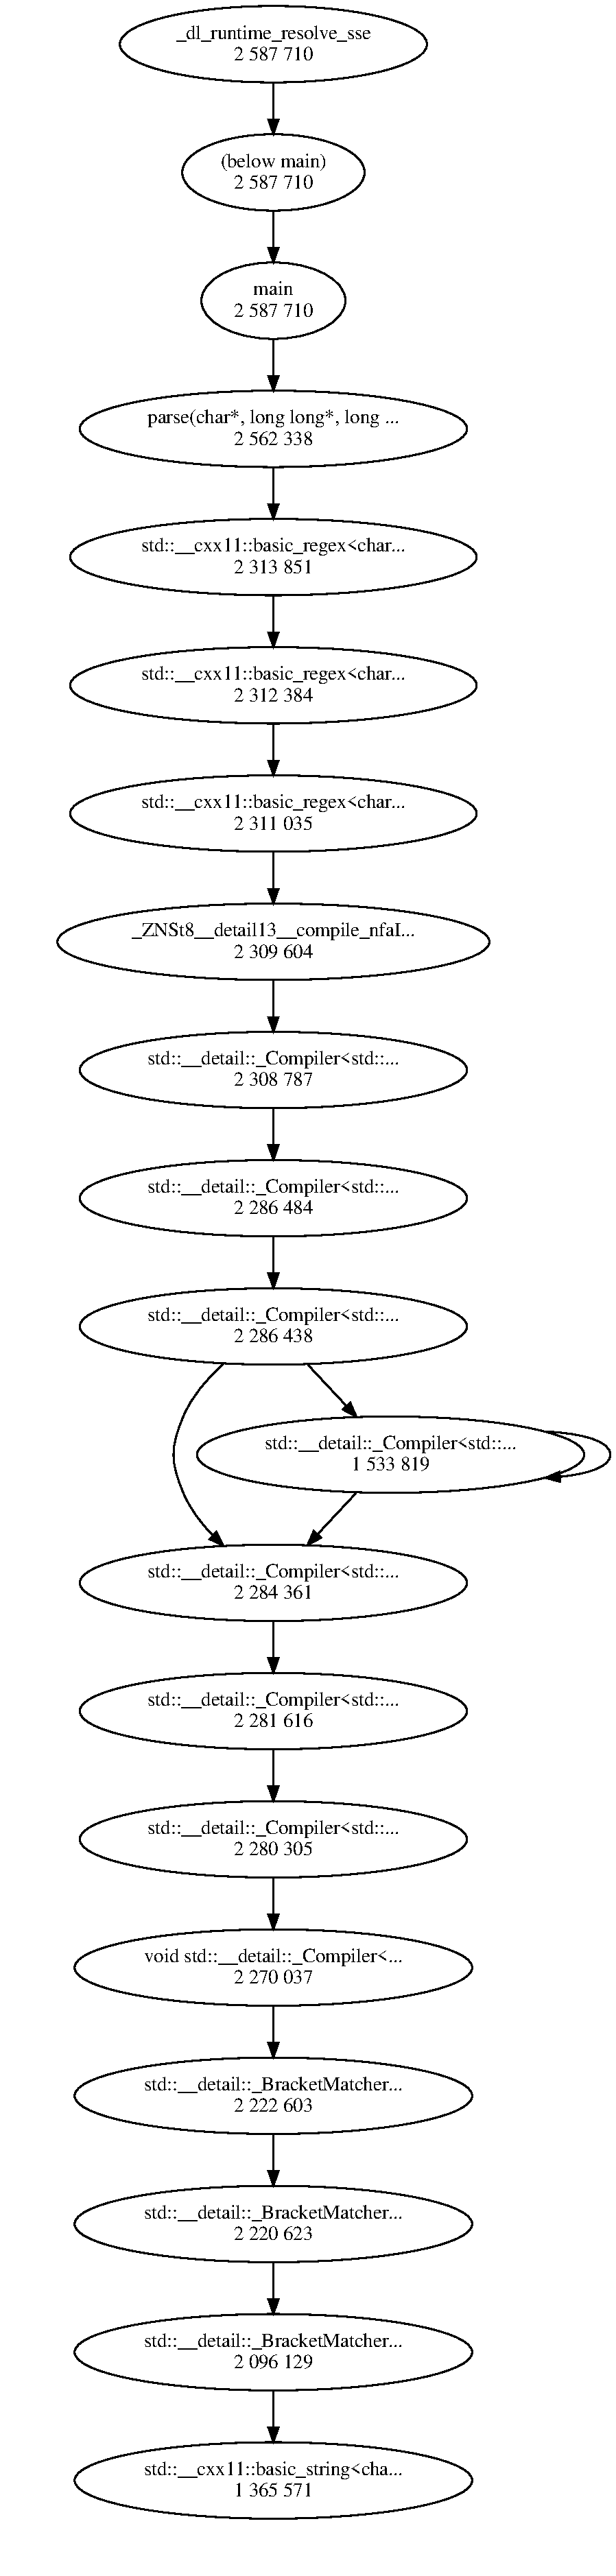
\includegraphics[width=0.33\textwidth]{res/callgraph}
  \caption{Граф вызовов до обфускации}
  \label{fig:myGraph}
\end{center}
\end{figure}

\newpage

Графов вызовов после обфускации (рисунок 2).

\begin{figure}[htp]
\begin{center}
  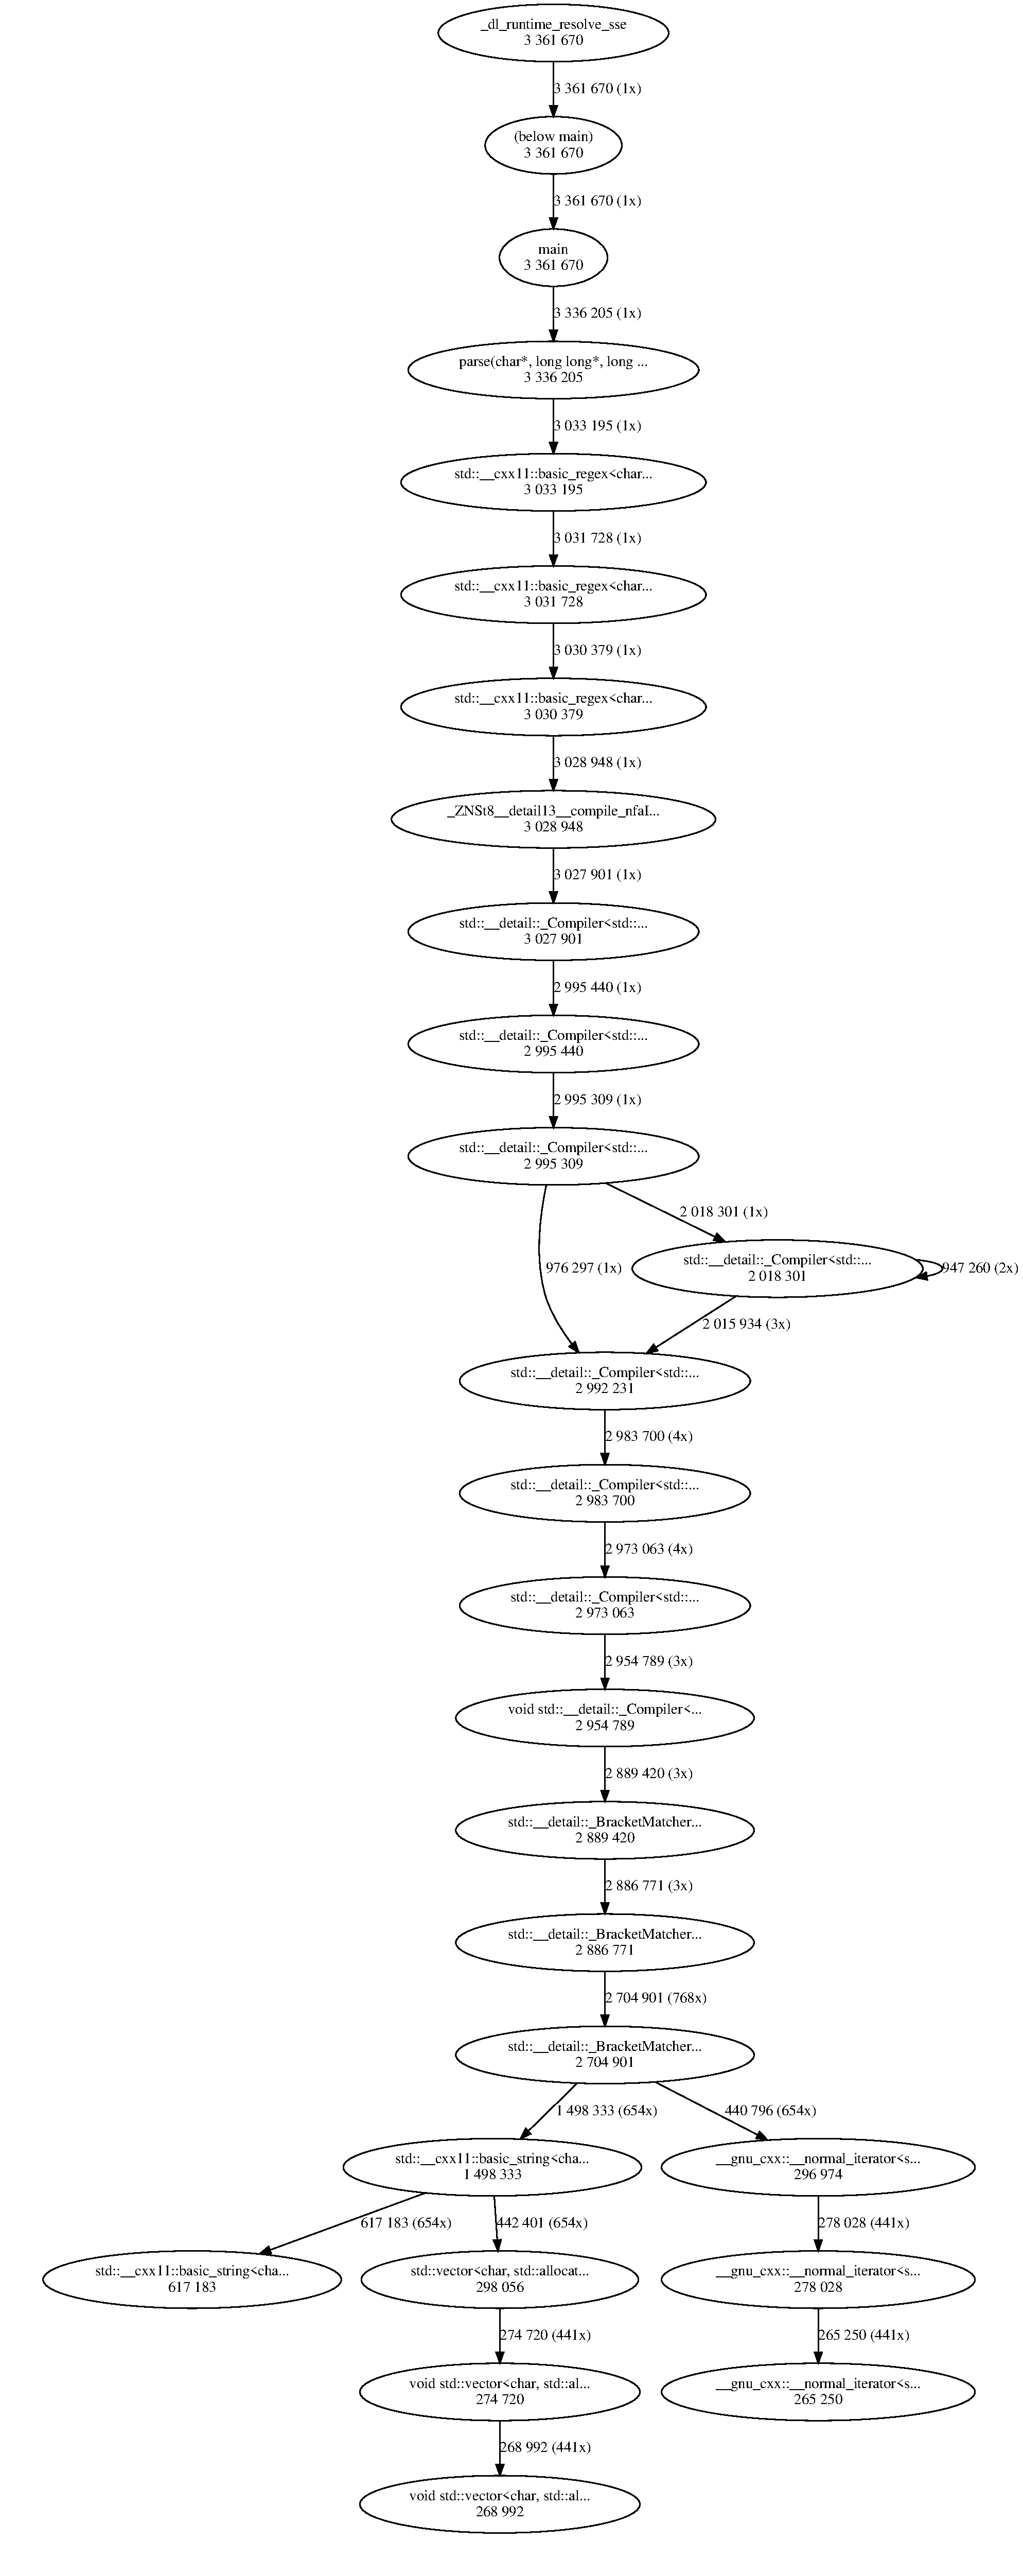
\includegraphics[width=0.41\textwidth]{res/callgraph2}
  \caption{Граф вызовов после обфускации}
  \label{fig:myGraph2}
\end{center}
\end{figure}

Как видно, графы достаточно похожи. Дело в том, что большая часть работы (парсинг строки с использованием регулярных выражений) происходит в стандартной библиотеке C++. Для повышения зашиты можно либо обфусцировать стандартную библиотеку, либо отказаться от её использования и переписать парсинг самостоятельно. Но та часть, которая отвечает за вывод информации, и которая как раз подверглась обфускации, отличается достаточно значительно. %

\newpage
%------------------------------------------------
\section*{Заключение}
\addcontentsline{toc}{section}{Заключение}

В данной работе были рассмотрены некоторые системные вызовы, используемые для управления планировщиком при работе с процессами реального времени (POSIX.1b).

В теоретической части было дано описание работы системных вызовов и работы планировщика; по умолчанию все процессы выполняются с интервалос времени равынм 100 мс и приоритетом (nice) 0, который слияет на интервал, позволяя изменять его в диапазоне от 10 мс до 200 мс.

В практической части приведён пример кода, вызывающего изучаемые системные вызовы. Перехват этих вызовов осуществлялся при помощи системной утилиты strace. % Заключение

\newpage
\section*{}
\addcontentsline{toc}{section}{Список литературы}

\begin{thebibliography}{00}

\bibitem{Love} Роберт Лав: «Разработка ядра Linux», Вильямс, 448 стр., 2008, ISBN
5-8459-1085-1, 0-672-32720-1.

\bibitem{Cragon} Harvey G. Cragon: «Computer Architecture and Implementation», Cambridge University Press, 238 pages, 2000, ISBN-10: 521651689.

\bibitem{Rosen} Rami Rosen: «Linux Kernel Networking: Implementation and Theory», Apress, 650 pages, 2014, ISBN-13: 978-1-4302-6196-4.

\bibitem{Realtech} Realtech: RTL8111B, Single-Chip Gigabit LOM Ethernet Controller for PCI Express. Datasheet Rev. 1.4, 02 December 2005, Track ID: JATR-1076-21.

\end{thebibliography} % Источники

%------------------------------------------------------------------------------

\end{document}